
\chapter{\IfLanguageName{dutch}{Stand van zaken}{State of the art}}%
\label{ch:stand-van-zaken}

% Tip: Begin elk hoofdstuk met een paragraaf inleiding die beschrijft hoe
% dit hoofdstuk past binnen het geheel van de bachelorproef. Geef in het
% bijzonder aan wat de link is met het vorige en volgende hoofdstuk.

% Pas na deze inleidende paragraaf komt de eerste sectiehoofding.
VMware ~\autocite{vmware} is een bedrijf dat zich specialiseert in virtualisatietechnologieën. De sterke prijsstijgingen van VMware zorgen ervoor dat veel bedrijven afhaken en op zoek gaan naar alternatieven ~\autocite{Hale2024}.
Er zijn verschillende alternatieve managementplatformen met bijhorende hypervisors.
In dit hoofdstuk wordt een overzicht gegeven van relevant onderzoek rond hypervisors en managementplatformen.
Eerst komen de verschillende hypervisors en managementplatformen aan bod, gevolgd door een bespreking van geschikte open-source en closed-source systemen en hun voor- en nadelen.
Vervolgens wordt ingegaan op de verschillende opslagoplossingen en de manier waarop deze in de hypervisors en managementplatformen geïntegreerd worden.
Daarna wordt de ondersteuning voor high availability behandeld, en tot slot wordt een samenvatting en vergelijking van de managementplatformen met bijbehorende hypervisors gepresenteerd, inclusief een analyse van hun prestaties.
\subsection{Hypervisors}\label{subsec:Hypervisors}
In het huidige systeem dat Excentis gebruikt, fungeert VMware ESXi ~\autocite{vmware} als onderliggende hypervisor. Deze is closed source en werkt binnen het VMware systeem. Als alternatief voor VMware ESXI zijn er verschillende hypervisors op de markt.

\begin{itemize}
    \item Een voorbeeld hiervan is 'KVM' (Kernel-based Virtual Machine) ~\autocite{KVM}. KVM is open source en vrij te gebruiken voor iedereen ~\autocite{KVM}.

    \item Microsoft Hyper-V ~\autocite{Eaton2019} wordt ook genoemd als mogelijke vergelijking met VMware ESXI~\autocite{fayyad2013benchmarking}. In dit onderzoek wordt een vergelijking gemaakt tussen verschillende hypervisors die geselecteerd zijn.

    \item Verder in de virtualisatiewereld bestaat ook het Xen Project ~\autocite{xenproject}. Dit is een open-source hypervisor die zich vooral richt op cloud computing en server virtualisatie~\autocite{binu2011virtualization}.

    \item XenServer ~\autocite{xenserverwebsite} (nu Citrix Hypervisor) is ook een alternatieve software keuze voor VMware ESXI. XenServer is een commerciële hypervisor die zich richt op bedrijven en enterprise-ondersteuning biedt.

    \item XCP-ng ~\autocite{el2021server} is een open-source hypervisor die is afgeleid van de Citrix Hypervisor (XenServer). Dit biedt een gratis alternatief voor bedrijven die op zoek zijn naar een hypervisor met enterprise-ondersteuning. XCP-ng ligt zeer dicht bij XenServer aangezien het een fork geweest is. Het wordt beheerd door de Linux Foundation en biedt op die manier een betrouwbare toekomst op verdere ontwikkeling en ondersteuning.
\end{itemize}

% Een voorbeeld hiervan is 'KVM' (Kernel-based Virtual Machine) \autocite{KVM}. KVM is open source en vrij te gebruiken voor iedereen \autocite{KVM}. Microsoft Hyper-V ~\autocite{Eaton2019} wordt ook genoemd als mogelijke vergelijking met VMware ESXI ~\autocite{fayyad2013benchmarking}. In dit onderzoek wordt een vergelijking gemaakt tussen verschillende hypervisors die geselecteerd zijn.
% Verder in de virtualisatiewereld bestaat ook het Xen Project ~\autocite{xenproject}. Dit is een open-source hypervisor die zich vooral richt op cloud computing en server virtualisatie ~\autocite{binu2011virtualization}.
% XenServer ~\autocite{xenserverwebsite} (nu Citrix Hypervisor) is ook een alternatieve software keuze voor VMware ESXI. XenServer is een commerciële hypervisor die zich richt op bedrijven en enterprise-ondersteuning biedt.
% XCP-ng ~\autocite{el2021server} is een open-source hypervisor die is afgeleid van de Citrix Hypervisor(XenServer). Dit biedt een gratis alternatief voor bedrijven die op zoek zijn naar een hypervisor met enterprise-ondersteuning.
% XCP-ng ligt zeer dicht bij XenServer aangezien het een fork geweest is. Het wordt beheerd door de linux foundation en bied op die manier een betrouwbare toekomst op verdere ontwikkeling en ondersteuning.

\subsection{Managementplatformen}\label{subsec:managementplatformen}
Excentis gebruikt als managementplatform VMWare vCenter~\autocite{vmware}. Voor dit platform moet een alternatief worden gevonden.

\begin{itemize}
    \item Proxmox VE~\autocite{Proxmox} is een open-source managementplatform dat werkt met KVM en enterprise-ondersteuning aanbiedt voor bedrijven. Uit onderzoek van \textcite{ally2018comparative} blijkt dat Proxmox, dat gebruik maakt van KVM, zeker niet onderdoet tegenover andere closed source systemen.

    \item OpenStack is een open-source cloud computing platform ~\autocite{openstack2024}.Deze biedt niet alleen ondersteuning voor KVM maar ook voor Xen~\autocite{oleksiuk2023comparative}.

    \item Microsoft System Center Virtual Machine Manager (SCVMM) ~\autocite{microsoftvmm2025} is een product van Microsoft en biedt een managementplatform systeem aan voor Hyper-V. Dit product bestaat nog maar in beperkte vorm en is niet meer meegegroeid met de node van een gemiddeld bedrijf.

    \item XenCenter ~\autocite{xencenter2024} is de officiële Windows‑client voor het beheren van XenServer, dat inmiddels Citrix Hypervisor heet~\autocite{xenserverwebsite}.

    \item Xen Orchestra ~\autocite{el2021server} is een open-source managementplatform dat werkt via een web interface. De gebruiker moet geen applicatie meer op de pc installeren. Het kan zowel clusters beheren van XCP-ng of Citrix Hypervisor/XenServer. Het kan gratis gebruikt worden tot een bepaald niveau. Support is mogelijk met een contract.
\end{itemize}
% Proxmox VE~\autocite{Proxmox} is een open-source managementplatform dat werkt met KVM en enterprise-ondersteuning aanbiedt voor bedrijven. Uit onderzoek van \textcite{ally2018comparative} blijkt dat Proxmox, dat gebruik maakt van KVM, zeker niet onderdoet tegenover andere closed source systemen.
% OpenStack is een open-source cloud computing platform~\autocite{openstack2024}. Het dient geïnstalleerd te worden individueel van je hypervisor. Het ondersteunt verschillende hypervisors zoals KVM en Xen.
% Deze biedt niet alleen ondersteuning voor KVM maar ook voor Xen~\autocite{oleksiuk2023comparative}.
% Microsoft System Center Virtual Machine Manager (SCVMM)~\autocite{microsoftvmm2025} is een product van Microsoft en biedt een managementplatform systeem aan voor Hyper-V. Dit product is helaas stopgezet en wordt niet meer ondersteund.
% XenCenter~\autocite{xencenter2024} is de officiële Windows‑client voor het beheren van XenServer, dat inmiddels Citrix Hypervisor heet~\autocite{xenserverwebsite}.
% Xen Orchestra ~\autocite{el2021server} is een open-source managementplatform dat werkt via een web interface. De gebruiker moet geen applicatie meer op de pc installeren. Het kan zowel clusters beheren van XCP-ng of Citrix Hypervisor/XenServer.
% Het kan gratis gebruikt worden tot een bepaald niveau. Support is mogelijk met een contract.
\subsection{Open source systemen}\label{subsec:opensource}
Er zijn vele soorten softwarepakketten op de markt die hypervisors en managementplatformen aanbieden. Bij het bekijken van de verschillende managementplatformen met hun bijbehorende hypervisors kunnen deze worden onderverdeeld in twee groepen: de closed-source en open-source hypervisors. Elke groep heeft zijn voor- en nadelen. Alles hangt steeds af van de noden en vereisten van het bedrijf of instelling.
Proxmox VE is open source~\autocite{Proxmox}. Dit wil zeggen dat de systemen kosteloos gebruikt kunnen worden. Support bij problemen valt hierbij wel af. Er is wel een mogelijkheid om bij hen een enterprise support services subscription te nemen. Hierbij kan er alsnog beroep worden gedaan op support bij eventuele problemen.
Open source software is een evidentie maar zorgt voor meer zelfstandig werk bij installatie en rust meer op de community achter de software.

\subsection{Closed source systemen}\label{subsec:clousedsource}
Andere alternatieven zijn closed-source. Hierbij gaat het onder andere om VMware ESXi/VMware vCenter~\autocite{vmware} en Microsoft Hyper-V~\autocite{Eaton2019}. Deze software systemen zijn niet gratis en vragen een licentie om te mogen gebruiken. Dit is een nadeel ten opzichte van open-source systemen.
Bij bedrijven waar stabiliteit en betrouwbaarheid hoog in het vaandel staan, zoals in een wetenschappelijke omgeving met supercomputers die veel geld kosten als ze niet draaien, kan het een goede keuze zijn om te kiezen voor closed-source hypervisors~\autocite{voras2012early}. Dit wil niet zeggen dat andere systemen uitgesloten zijn.


\subsection{Soorten storage systemen}\label{subsec:storage}
Wanneer het over opslag in de virtualisatiewereld gaat, betreft het ook 'Serial-Attached SCSI' (SAS) en 'Direct-Attached Storage' (DAS). Deze technologieën zorgen ervoor dat er een hoge beschikbaarheid is van de data en dat deze snel kan worden opgevraagd~\autocite{griswold2002storage}. Dit is een belangrijk aspect in de virtualisatiewereld en het is belangrijk voor Excentis dat deze beide technologieën perfect werken en ondersteund worden.
SAS is een snelle, betrouwbare opslaginterface die servers en high-performance opslagapparaten verbindt~\autocite{aravindan2014performance}. Dit is belangrijk om een consistente opslag te garanderen. DAS is een opslagarchitectuur waarbij opslag direct fysiek is verbonden aan een enkele server, zonder tussenkomst van een netwerk. Deze technologie is goedkoper en eenvoudiger, maar garandeert niet alle voordelen die SAS wel kan bieden~\autocite{griswold2002storage}.
DAS wordt veel gebruikt in consumententoestellen zoals laptops en desktops. SAS daarentegen wordt hoofdzakelijk toegepast in serversystemen waar data essentieel is en een hoge betrouwbaarheid en performantie vereist is~\autocite{griswold2002storage}.
In dit onderzoek blijkt dat vrijwel alle managementplatformen ondersteuning bieden voor zowel DAS als SAS. Excentis wenst na te gaan hoe deze ondersteuning efficiënt kan worden gemigreerd naar een nieuw managementplatform.

Storage Area Network (SAN) \textcite{ibm2025san} is een technologie die gebruikt wordt om storage te delen over het netwerk.
Dit is puur een manier om storage op te zetten. \\
Je hebt hiernaast ook nog een protocol of manier nodig om te kunnen communiceren met de storage op die server.
Daar zijn er voornamelijk 2 toepassingen voor: iSCSI en FC (Fibre Channel).
In het onderzoek van \textcite{stonefly2023fcvsiscsi} wordt er gesproken over iSCSI en FC met hun bijhorende voor en nadelen. Dit zijn twee veel gebruikte protocollen voor niet direct attach storage systemen.

\begin{itemize}
    \item iSCSI (Internet Small Computer System Interface) is een protocol dat SCSI-commando's over IP (layer 3) verzendt. Het maakt gebruik van TCP/IP om opslagapparaten te verbinden met servers en opslag via een netwerk. Dit maakt het mogelijk om opslagbronnen op afstand te delen en te beheren, wat de flexibiliteit en schaalbaarheid vergroot. Het is makelijk toe te passen met standaard netwerkapparatuur en is relatief goedkoop in vergelijking met andere opslagprotocollen. Het grootste nadeel is dat de latency hoger is dan bij FC, omdat het gebruik maakt van TCP/IP en dus afhankelijk is van de netwerkprestaties.
    \item FC (Fibre Channel) is een hoogwaardig netwerkprotocol dat speciaal is ontworpen voor opslagnetwerken. Het nadeel met dit systeem is dat er speciale netwerk apparatuur nodig is om dit protocol te kunnen gebruiken. Deze hardware is ook duur. Het grootste voordeel is wel dat er een veel lagere latency is dan bij iSCSI. 
\end{itemize}


\subsection{High Availability-ondersteuning}\label{subsec:ha}
In het onderzoek van~\textcite{dudnik2017creating} wordt een grote vergelijking gemaakt tussen hypervisors en hun managementplatformen. Hierin wordt gefocust op bepaalde aspecten binnen de term High Availability, zoals redundantie, risicoanalyse en piekdrukte.
Er zijn verschillende aspecten die moeten worden bekeken en waaraan voldaan moet worden om aan een goede High Availability te voldoen. Een failover-systeem dat het ene systeem het andere systeem over laat nemen bij een bepaalde fout, is één van die aspecten.
Op netwerkniveau moet er ook nagedacht worden over zowel schaalbaarheid bij piekmomenten als bij problemen die zich voordoen in het netwerk. Migratie tussen verschillende fysieke servers moet ook mogelijk zijn om een goede High Availability te garanderen~\autocite{dudnik2017creating}.
Workloadmanagers kunnen een goede oplossing zijn om overbelasting tegen te gaan op drukke piekmomenten. Back-ups van de data worden ook gezien als een belangrijk aspect voor High Availability.


\subsection{Samenvatting van alle managementplatformen en hun bijhorende hypervisors als long-list}\label{subsec:samenvatting}
In tabel~\ref{tab:longlist} wordt een overzicht gegeven van de verschillende hypervisors en hun bijhorende managementplatformen. Dit is een long-list van de verschillende systemen die in dit onderzoek aan bod komen. Hierop wordt er nog geselecteerd welke in aanmkerking komen voor de proof of concept.

    \begin{table}[h!]
        \centering
        \small
        \begin{tabular}{|p{2cm}|p{2cm}|p{3cm}|p{7cm}|p{7cm}|}         
        \hline
        \textbf{Platform}      & \textbf{Type}      & \textbf{Hypervisor} & \textbf{Description} \\ \hline      
        VMware vCenter         & Closed-source      & VMware ESXi         & Enterprise management platform voor VMware-gebaseerde virtualisatie. \\ \hline
        Microsoft SCVMM        & Closed-source      & Microsoft Hyper-V   & Beheert Hyper-V-omgevingen en biedt integratie met andere Microsoft-producten. \\ \hline
        Proxmox VE             & Open-source        & KVM                 & Geavanceerd open-source managementplatform voor KVM, met enterprise-ondersteuning. \\ \hline
        OpenStack              & Open-source        & KVM, Xenserver, VMware, of Hyper-V,...  & Cloud computing-platform dat meerdere hypervisors ondersteunt. \\ \hline
        Xen Project            & Open-source        & Xen                 & Managementplatform dat Open-source is. \\ \hline
        Xen Orchestra  & Open-source & XCP-ng,Citrix Hypervisor(xenserver)  & opvolger XEN project \\ \hline
        Xen Center  & Closed-source & Citrix Hypervisor(xenserver)   &  Betalende versie met enterprise support\\ 
       \bottomrule        
        \end{tabular}
        \caption{Vergelijking van Virtualisatieplatformen}
        \label{tab:longlist}        
        \end{table}
\clearpage        
\subsection{Prestatie verschillen tussen managementplatformen} \label{subsec:performace}
In het onderzoek van \textcite{algarni2018performance} wordt een vergelijkende studie gemaakt tussen Xen en KVM. In ons onderzoek focussen wij ons vooral op het managementplatform.
Aangezien een managementplatform ook een hypervisor nodig heeft kunnen wij hier spreken over het management platform die gekoppeld is in deze studie aan een hypervisor.
Voor KVM wordt er gesproken over PROXMOX VE en voor Xen wordt er gesproken over XenServer. In deze studie wordt er een vergelijking gemaakt tussen de twee systemen en hun prestaties. De resultaten zijn als volgt:
Over het volledige onderzoek van \textcite{algarni2018performance} heen krijgt KVM (gekoppeld aan Proxmox VE voor ons onderzoek) de beste punten over het globale punt heen. Dit onderzoek heeft plaats gevonden in 2018 waarbij de conclusies nog als actueel kunnen beschouwd worden.
Dit is een belangrijk onderzoek om conclusies uit te trekken eenmaal een proof of concept gemaakt is. \\
OpenStack is een buitenbeentje in deze longlist. OpenStack is specifiek bedoeld voor te werken als cloud oplossing. In het onderzoek van \textcite{callegati2014performance} wordt er duidelijk getoont dat het gemaakt is voor cloudoplossingen. Eventueel met een hybride could oplossing. \\
Microsoft SCVMM ~\autocite{microsoftvmm2025}  is een product van Microsoft en biedt een managementplatform systeem aan voor Hyper-V. Uit het onderzoek van \textcite{fayyad2013benchmarking} blijkt dat Hyper-V over het geheel genomen gemiddeld presteert. \\
Xen Orchestra is een recenter product die werkt met de nieuwe XCP-ng hypervisor. Dit is een fork van XenServer. In het onderzoek van \textcite{el2021server} wordt Xen Orchestra die gebruik maakt van Citrix XenServer als beste uit het onderzoek gehaald waarbij het globaal gezien beter presteert dan KVM die gebruikt wordt door Proxmox VE \\

\begin{itemize}
    \item \textbf{Proxmox VE (KVM)} heeft een betere prestatie in termen van CPU‑gebruik en geheugengebruik dan XenServer.
    \item \textbf{Citrix XenServer} (zoals gebruikt door Xen Orchestra) heeft een betere prestatie in termen van I/O‑prestaties dan Proxmox VE, met name bij bestandssysteembeheer en applicatie‑respons.
    \item \textbf{OpenStack} is specifiek ontworpen als cloud‑ en (hybride) cloud‑oplossing; het biedt uitstekende schaalbaarheid en flexibiliteit, maar introduceert wel extra overhead waardoor de ruwe CPU‑ en geheugendurchvoer iets lager ligt dan bij Proxmox VE of XenServer \autocite{callegati2014performance}.
    \item \textbf{Microsoft SCVMM (Hyper‑V)} heeft volgens benchmarks een gemiddelde algehele prestatie; het positioneert zich tussen Proxmox VE en XenServer in, met degelijke netwerk‑ en opslagdoorvoersnelheden, maar gemiddeld CPU‑gebruik.
    \item \textbf{Xen Orchestra (XCP‑ng)} – een fork van XenServer – profiteert van de verbeteringen in Citrix XenServer en behaalt in onderzoek de beste totaalscores, met name op CPU‑, geheugen‑ en netwerkniveaus, beter dan Proxmox VE (KVM).
\end{itemize}
                               

\subsection{Storage ondersteuning voor hypervisors en managementplatformen}\label{subsec:storageondersteuning}

Zoals eerder uitgelegd wordt er in dit onderzoek gekeken naar Serial-Attached SCSI (SAS) en Direct-Attached Storage (DAS). Deze technologieën zijn belangrijk voor de virtualisatiewereld en zijn ook belangrijk voor Excentis. Het is belangrijk dat deze technologieën goed werken met de hypervisors en managementplatformen die in dit onderzoek worden bekeken.
Om in de proof of concept deze technologieën te kunnen gebruiken moet er gekeken worden of elk managementplatform deze technologieën ondersteunt.
SAS-storage staat los van elke hypervisor met hun bijhorende virtual managementplatformen. Het is een technologie die gebruikt wordt om storage te delen over het netwerk. Dit is puur een manier om storage op te zetten. Je hebt hiernaast ook nog een protocol of manier nodig om te kunnen communiceren met de storage op die server.
Afbeelding ~\ref{fig:sas} toont een volledig beeld van SAS-systemen. Dit is een afbeelding die de kracht van SAS-systemen weergeeft. Het laat zien dat SAS tot 2 keer zoveel meer data kan versturen en verwerken t.o.v. het bekende SATA systeem.
\begin{figure}[h!]
    \centering
    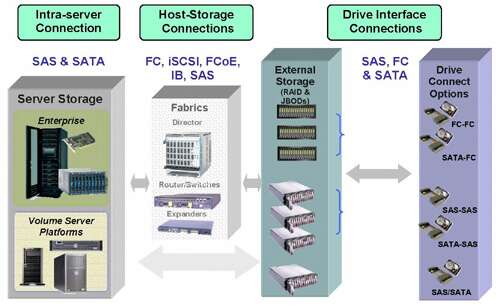
\includegraphics[width=0.7\textwidth]{../onderzoek/storagesas-das.jpg} 
    \caption{volledig beeld die SAS weergeeft, afkomstig van \textcite{eetimesSAS}}
    \label{fig:sas}
\end{figure}

\FloatBarrier
Figuur~\ref{fig:saspres} toont de kracht van SAS systemen. In het artikel van \textcite{loshin2022sas} wordt er uitgelegd dat SAS tot 2 keer zoveel meer data kan versturen en verwerken t.o.v. het bekende SATA systeem.

\begin{figure}[h!]
    \centering
    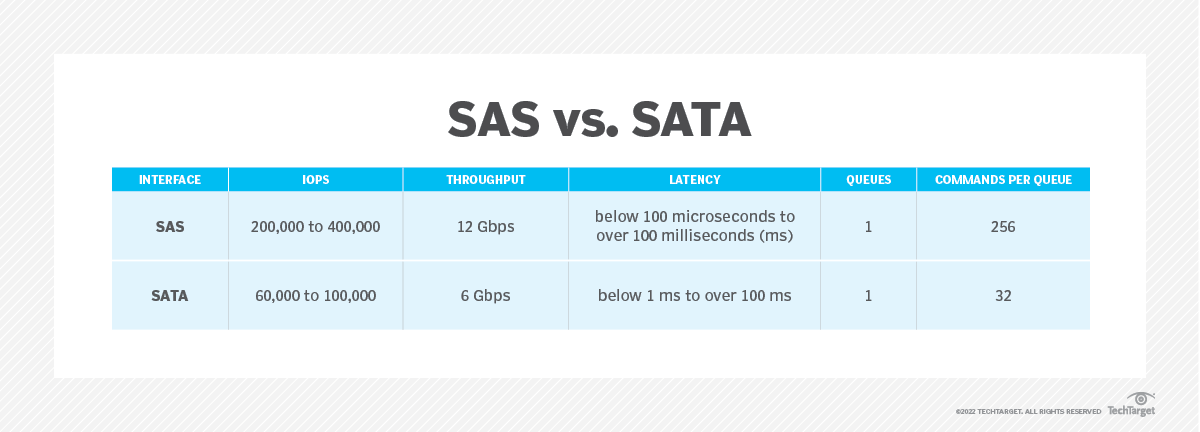
\includegraphics[width=1.1\textwidth]{../onderzoek/sas_vs_sata-f.png} 
    \caption{Afbeelding die SAS prestatie weergeeft, afkomstig van \textcite{loshinKranzSAS} over Serial Attached SCSI.}
    \label{fig:saspres}
\end{figure}


\FloatBarrier
Verder wordt er ook nog Storage Area Network (SAN) gebruikt in combinatie met iSCSI voor grote storage-opslagsystemen. In het onderzoek van \textcite{park2024performance} wordt besproken hoe iSCSI een positieve invloed heeft op de prestatie van storagesystemen die gedeeld worden met verschillende toepassingen.
Figuur ~\ref{fig:san} toont een afbeelding die SAN weergeeft.
In het bedrijf Excentis is het daarom ook belangrijk dat de storage van het virtual managementplatform gedeeld kan worden met verschillende toepassingen. Bij het onderzoek van \textcite{park2024performance} wordt bevestigd dat dit een goede standaardmethode is voor storage over het netwerk.
ISCI is hiermee ook een belangrijk punt om rekening mee te houden in de proof of concept. Het is belangrijk dat de iSCSI goed werkt met de hypervisors en managementplatformen die in dit onderzoek worden bekeken.

\begin{figure}[h!]
  \centering
  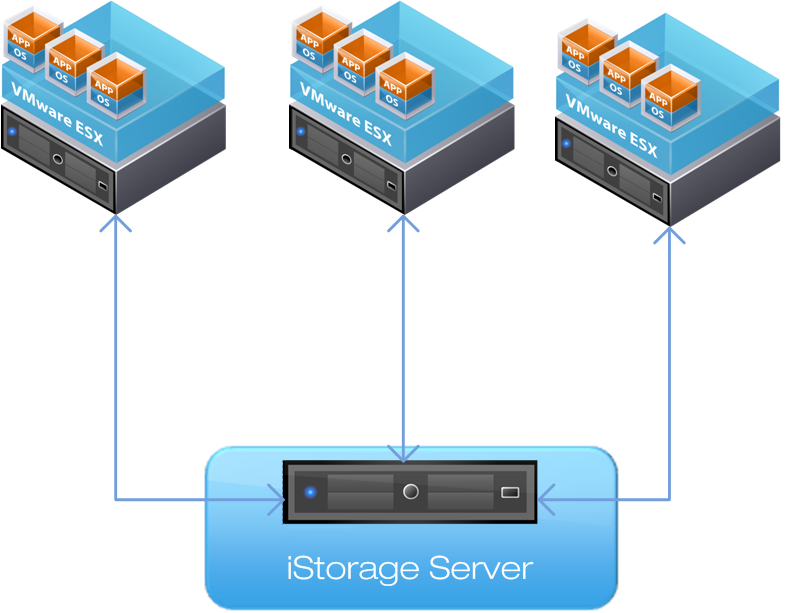
\includegraphics[width=0.7\textwidth]{../onderzoek/nas-isci.png} 
  \caption{Afbeelding die SAN simpel weergeeft, afkomstig van \textcite{kernsafeVMware}.}
  \label{fig:san}
\end{figure}


\FloatBarrier
Bij DAS-systemen wordt, zoals eerder vermeld, de data rechtstreeks aan de hardware verbonden. Het onderzoek van \textcite{joshi2014empirical} richt zich specifiek tot schijfformaten op DAS-systemen.
Dit gaat buiten de scope van dit onderzoek, maar toont zeer mooi aan dat KVM (voor ons Proxmox VE) zeer goede ondersteuning biedt en hierbij ook aantoont dat er zeer veel ondersteunende schijfformaten bestaan.
Het is zeer moeilijk om correcte wetenschappelijke artikels te vinden over de implementatie van DAS- en SAS-systemen op alle soorten managementplatformen.
Er wordt vaak specifiek gericht op een gebruikt systeem die zich onder de categorie bevindt DAS of SAS. Het onderzoek van \textcite{joshi2014empirical} is daar een goed voorbeeld van.
Met de referenties en kennis die hieruit zijn gekomen, weten we dat DAS en SAS globaal over alle managementplatformen ondersteund worden. De afbeelding ~\ref{fig:das} toon overzichtelijk DAS ten opzichte van NAS en SAN.
De uitvoering en de praktische ervaring zal in de proof of concept worden bekeken. Daaruit moet uitkomen of de SAS- en DAS-integratie voldoende stabiliteit biedt.

\begin{figure}[h!]
    \centering
    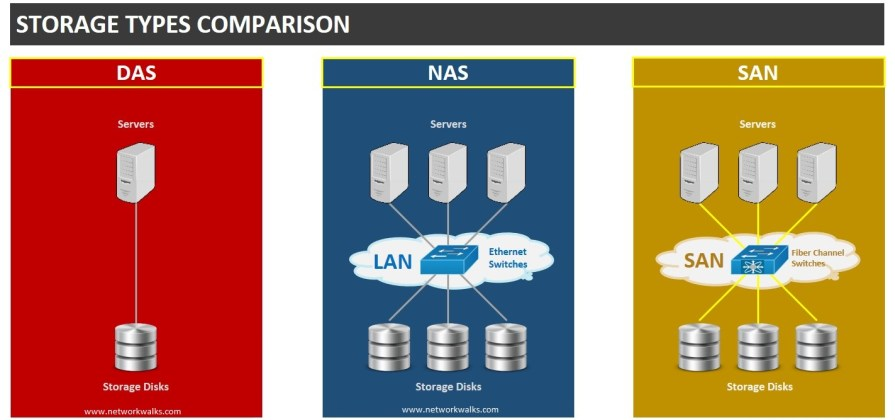
\includegraphics[width=0.7\textwidth]{../onderzoek/DAS.jpg} 
    \caption{Afbeelding die DAS simpel weergeeft, afkomstig van \textcite{tekmart2020nasvsdas}}
    \label{fig:das}
\end{figure}
\FloatBarrier
Gedistribueerde opslag of distributed storage is nog een belangrijke optie die toepasselijk is voor een virtual managementplatform. Dit is een opslagmethode waarbij de data over verschillende servers (nodes) wordt verdeeld.
Dit zorgt ervoor dat de data sneller kan worden opgevraagd en netwerk verkeer efficiënt benut wordt. ~\autocite{patil2010unified}.
In het onderzoek zijn wij specifiek gefocust op toepassingen voor management platformen. VMware heeft zijn eigen private toepassing genaamd vSAN~\autocite{hogan2016essential}. Dit is een software-defined storage oplossing die speciaal is ontworpen voor VMware-omgevingen. Het biedt een effectieve opslagoplossing die eenvoudig kan worden geïntegreerd met VMware's virtualisatieplatformen.
Hierbij moet er dus ook een alternatief ter beschikking zijn. Eén daarvan die open source is, is Ceph~\autocite{weil2006ceph}. Dit is een open-source software-defined storage oplossing die kan worden gebruikt met verschillende managementplatformen zoals Proxmox VE ~\autocite{Proxmox}.

Bij figuur \ref{fig:das} is een theoretisch voorbeeld aangetoond. Ceph zelf en vSAN kan vergeleken worden met dit theoretisch voorbeeld.
\begin{figure}[h!]
  \centering
  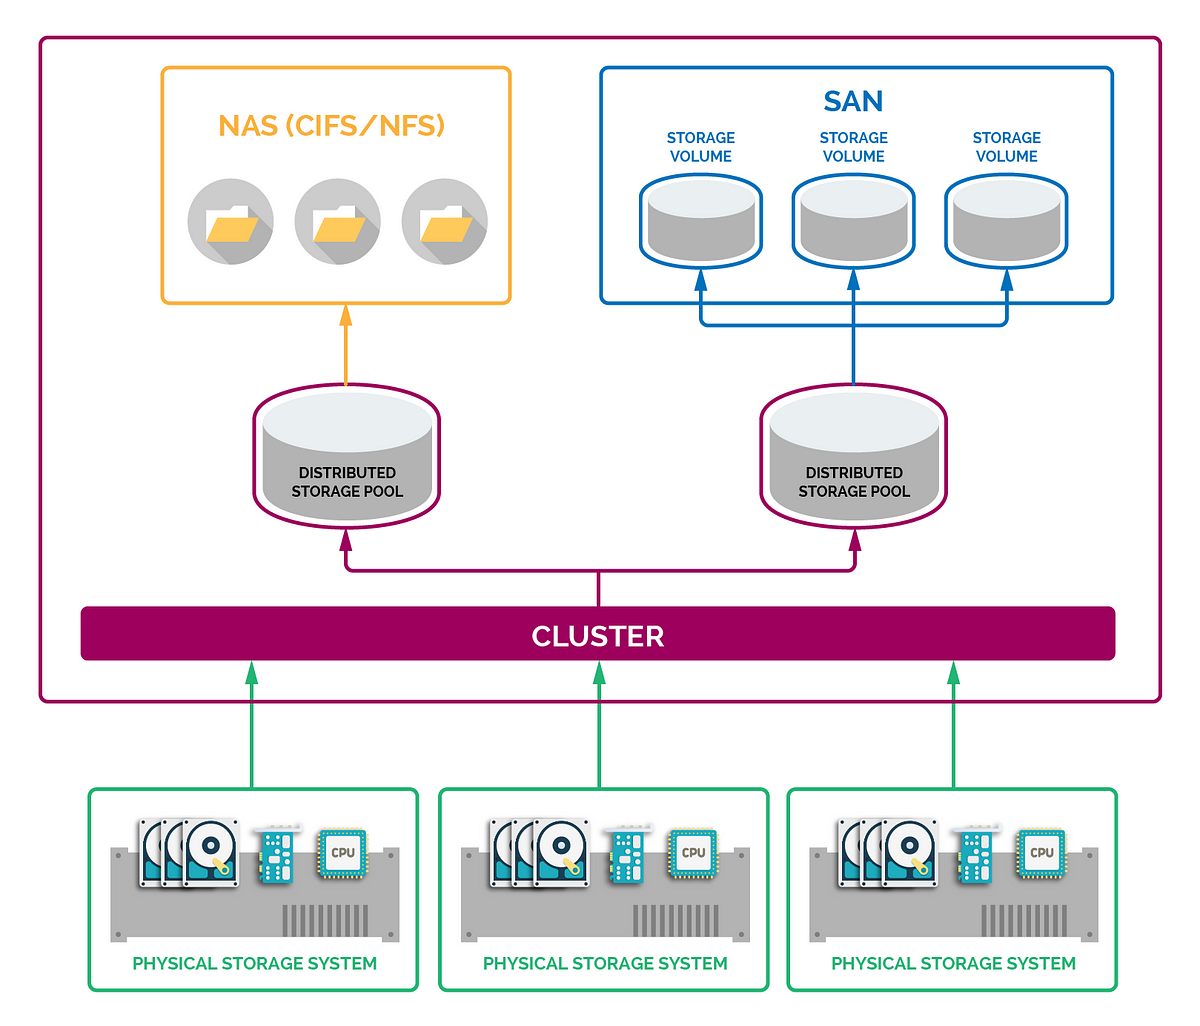
\includegraphics[width=0.9\textwidth]{../onderzoek/dssep.png} 
  \caption{Afbeelding van distributed storage als toepassing., afkomstig van \textcite{pb2022storage}.}
  \label{fig:das}
\end{figure}

Xen Orchestra heeft ook zijn eigen distributed storage-oplossing genaamd XOSTOR~\autocite{xostor-docs}. Dit is een software-defined storage-oplossing die speciaal is ontworpen voor XCP-ng en Xen Orchestra. Het biedt een opslagoplossing als virtuele SAN die eenvoudig kan worden geïntegreerd met XCP-ng en Xen Orchestra.
Het is zeer vergelijkbaar met CEPH~\autocite{weil2006ceph}, dat ook werkt met schijven die in de cluster zitten. Beide zorgen ervoor dat de fysieke disks op alle nodes onderling voor elkaar beschikbaar zijn. Er wordt ook aan replica’s gedaan waarbij er een RAID-achtige manier wordt toegepast.
Als er een schijf verloren gaat, zal een andere het overnemen. De enige voorwaarde is bij XOSTOR en CEPH dat er minimaal 3 schijven beschikbaar zijn.